\begin{refsection}
\renewcommand{\thefigure}{\arabic{figure}}

\chapterTwoLines
{Não ao peso, não ao recrutamento}
{os Quebra-quilos e as autoridades públicas no Rio Grande do Norte (1874--1875)}
\label{chap:naoaopeso}

\articleAuthor
{João Fernando Barreto de Brito}
{Doutor pelo Programa de Pós-Graduação em História Social da Universidade Federal do Rio de Janeiro (PPGHIS/UFRJ). ID Lattes: 2836.1238.5025.4834. ORCID: 0000-0003-1692-8703, e-mail: joaofernandohistoria@gmail.com.}

\begin{galoResumo}
    \marginpar{
        \begin{flushleft}
        \tiny \sffamily
        Como referenciar?\\\fullcite{SelfBrito2021}\mybibexclude{SelfBrito2021}, p. \pageref{chap:naoaopeso}--\pageref{chap:naoaopesoend}, \journalPubDate{}
        \end{flushleft}
    }
    No ano de 1874 as notícias sobre as ações dos Quebra-quilos circulavam com grande velocidade na província do Rio Grande do Norte. As feiras, casas comerciais e tabernas eram espaços privilegiados para a disseminação das fofocas e mexericos em torno de uma onda de revoltas nascidas no interior da Paraíba do Norte. A cada momento, notícias chegavam aos ouvidos de autoridades públicas, mas também de pessoas que se mostraram insatisfeitas com a política imperial, com os impostos municipais, com o recrutamento por sorteio e, sobretudo, com a lei que estabeleceu oficialmente o Sistema Métrico Decimal Francês (SMD), substituindo as tradicionais costumeiras medidas antropométricas lusitanas, prevendo multa e prisão para aqueles que ousassem desrespeitar tal determinação. O presente artigo investigou a atuação dos Quebra-quilos no Rio Grande do Norte, destacando vilas e povoações atingidas por esses sediciosos, identificando os grupos sociais partícipes, suas estratégias, e a maneira pela qual as autoridades públicas e militares combateram os revoltosos na citada província. Problematizamos fontes oficiais, correspondências, códices, periódicos de época e ofícios do governo Imperial. 
\end{galoResumo}

\galoPalavrasChave{Quebra-quilos. Sistema métrico decimal. Rio Grande do Norte.}

\begin{otherlanguage}{english}

\fakeChapterTwoLines
{No to weight, no to recruitment} {The Quebra-quilos rebels and public authorities in Rio Grande do Norte (1874--1875)}

\begin{galoResumo}[Abstract]
    In the year 1874, news about the actions of Quebra-Quilos rebels spread out quickly in the province of Rio Grande do Norte. Street markets, commercial houses and taverns were privileged spaces for spreading rumors and gossip about a wave of revolts started in the countryside of Paraíba do Norte. At every moment news reached public authorities, but it also echoed in sectors of society who were dissatisfied with imperial policy, municipal taxes, recruitment by drawing lots, and most of all the law that officially established the French Decimal Metric System (SMD), replacing the traditional customary Portuguese anthropometric measures and imposing fine and imprisonment for those who dared to disrespect such determination. The present article investigates the actions of Quebra-quilos in Rio Grande do Norte, highlighting the villages and towns affected by these seditious people, identifying the participating social groups, their strategies, and the way public and military authorities fought the rebels in that province. We problematize official sources, correspondences, codices, press reports of that time and official letters by the Imperial government.
\end{galoResumo}

\galoPalavrasChave[Keywords]{Quebra-quilos. Decimal Metric System. Rio Grande do Norte.}
\end{otherlanguage}

\section{Introdução}

Já nos últimos dias do mês de novembro de 1874, povoações e vilas do interior paraibano e pernambucano foram atacados pelos Quebra-quilos.\footnote{É possível compreender o significado atribuído na época à palavra “quebra-quilos” a partir da visão do Imperador Dom Pedro II, demonstrada em sua “Falla do Throno” diante da assembleia geral em 16 de março de 1875, oportunidade em que ordem pública novamente havia sido perturbarda, desta vez no interior de quatro províncias do Norte, perpetradas por “bandos sediciosos, em geral movidos por fanatismo religioso e preconceitos contra a pratica do systema metrico, assaltaram povoações, e destruiram archivos e padrões dos novos pesos e medidas”. Esta maneira de enxergar os seus súditos descontentes de certo servia como forma de deslegitimar a ação dos revoltosos, de modo que não reconhecia as reclamações e protestos proferidos por tais. Por outro lado, estigmatizava-os como “bandos sediciosos”, fazendo-se alusão a grupos de salteadores, estes impulsionados pela ignorância, por não aceitarem o sistema métrico imposto pelo governo, tresloucados religiosos, ou seja, que não agiam motivados pela razão. Ver SENADO FEDERAL. \textbf{Biblioteca Digital}. Falla do Throno na abertura da assembléa geral de 16 de março de 1875. Disponível em: <http://www2.senado.leg.br/bdsf/item/id/227319>, acessado em 29 de julho de 2016.} Feiras locais, casas comerciais, paróquias, coletorias e até as residências de pessoas influentes dessas localidades (juízes, coletores de rendas, subdelegados e delegados) foram alvos desses revoltosos. A situação entre os do \textit{mundo do governo} era de preocupação. Na província do Rio Grande do Norte adotaram-se medidas “preventivas”, prepararam-se com a finalidade de conter os agitadores. Oito dias após as primeiras agitações verificadas na província de Pernambuco, o Rio Grande do Norte recebeu da Secretaria dos Negócios de Guerra uma considerável quantidade de armamento. Parecia que os representantes provinciais sabiam da inevitabilidade dos conflitos e \textit{armaram-se até os dentes}, como diz o ditado popular. 

Mais de 22 mil utensílios a serem usados em combates desembarcaram em Natal, de onde seriam distribuídos para aqueles responsáveis por evitar o furor dos Quebra-quilos. O envio de espingardas raiadas, cartuchos, cápsulas, bornais entre outros objetos é de fato resultado do conhecimento prévio das autoridades acerca da proximidade dos confrontos com os Quebra-quilos.\footnote{ARQUIVO NACIONAL (Brasil), Código NP, Fundo ``Diversos códices da antiga SDH''. Notação do documento “Códice 603 v. 5”. Dr. José Maria Lopes da Costa, Secretaria do Estado dos Negócios de Guerra, em 29 de novembro de 1874, p. 24.}

Outra medida de prevenção articulada pelas autoridades do Rio Grande do Norte foi tomada ainda em 4 de dezembro de 1874, conforme publicou o jornal D. Pedro II, quando “partio o chefe de polícia Dr. Luiz Ignacio Barreto com destino á comarca de S. José e a diversos pontos da de Canguaretama, limitrophes da província da Parahyba, no intuito de providenciar em ordem a prevenir a invasão dos insurgentes daquella província”.\footnote{BIBLIOTECA NACIONAL (Brasil). \textbf{Hemeroteca Digital}. D. Pedro II, n. 34, 24 de dezembro de 1874, p.2. }

Um dia depois, Bandeira de Mello ainda demonstrava preocupação em relação a proteção da província, de modo que solicitou ao presidente pernambucano Henrique Pereira de Lucena, em virtude da “falta de armamento no Deposito de artigos belicos d’esta Província”,\footnote{Arquivo Público do Estado de Pernambuco Jordão Emerenciano [APEJE] --- Coleção correspondências entre presidentes de província, PP 53,1874, p. 290.} mais armamentos tendo em vista às “occurrencias que se vão dando na Província da Parahyba e de que se acham ameaçadas alguns pontos desta”.\footnote{Ibidem.} Naquele mesmo mês, em dia de 5 de dezembro de 1874, as previsões se confirmaram e aos poucos vários lugares seriam também palco das ações dos Quebra-quilos, como podemos observar da figura \ref{fig:quebra-quilo-rn}. 

\begin{figure}[ht]%
    \centering%
    \caption{Quebra-quilos no Rio Grande do Norte}%
    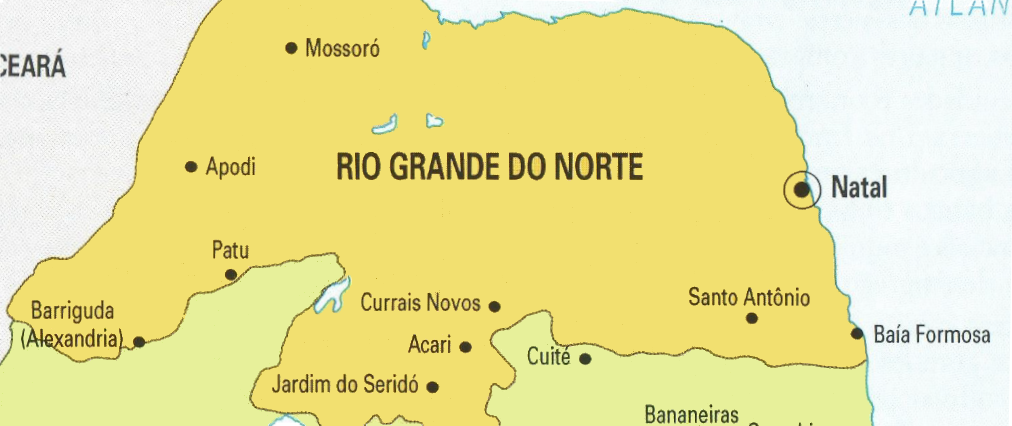
\includegraphics[width=.75\textwidth]{arcticles/02-nao-ao-peso-nao-ao-r/01-rn.png}%
    \caption*{Fonte: \textcite[p.~17]{Monteiro1993}}%
    \label{fig:quebra-quilo-rn}%
\end{figure}%

O presente artigo visa investigar a atuação dos Quebra-quilos no Rio Grande do Norte. Destacaremos as vilas e povoações atacadas por esses sediciosos, que grupos sociais participaram ativamente, quais estratégias foram utilizadas por eles, e como as autoridades públicas e policiais norte-rio-grandenses lidaram com esta que foi a maior revolta popular do século XIX. Serão investigadas fontes oficiais do governo, tais como correspondências entre presidentes de províncias, o códice 603 (fonte que reuniu vários documentos ministeriais da Guerra e da Justiça sobre a revolta), além de diversos periódicos. Analisaremos os discursos e falas das autoridades, bem como problematizaremos as ações, experiências e estratégias dos Quebra-quilos.

\section{Desenvolvimento}

Segundo a folha noticiosa \textbf{Diário de Pernambuco}, insurgentes da Paraíba transpassaram os limites provinciais e adentraram o Rio Grande do Norte em 5 dezembro de 1874. De acordo com o referido jornal, cerca 200 indivíduos denominados “quebra-kilos”, que unidos a mais 100 pessoas do lugar invadiram a feira da povoação de Santo Antônio, município de Goianinha, causando a destruição de pesos e medidas do SMD em diferentes estabelecimentos. Destacava a mencionada folha noticiosa, pretendiam os sediciosos adentrar a casa do padre capelão com o intuito de queimarem os livros de batismo dos filhos livres de mulheres escravas, algo não realizado posto que foram demovidos de suas intenções pelo subdelegado local.\footnote{BIBLIOTECA NACIONAL (Brasil). \textbf{Hemeroteca Digital}. Diário de Pernambuco, ed. 286, 15 de dezembro de 1874, p. 1.}

Ao atacarem a povoação de Santo Antônio (RN), os sediciosos usaram de estratégias já bem conhecidas, repetindo-se o \textit{modus operandi} das ações tidas nas províncias da Paraíba e Pernambuco. Parece-nos que a experiência dos ataques passados ainda na região da Borborema norteou as investidas tanto do lado pernambucano quanto do lado rio-grandense. A feira se manteve como espaço de aglutinação de novos revoltosos (dos paraibanos com os nativos) e o lugar de demonstrar as insatisfações com as políticas e autoridades imperiais. Isto porque a escolha de um alvo limítrofe à Paraíba não era algo aleatório. Os insurgentes paraibanos “invadiram” Santo Antônio e somaram-se a mais indivíduos deste povoado.

É preciso trazer à tona também a participação ativa de sujeitos pardos, caboclos e negros (escravos(as), ex-escravos(as) e gente livre) em algumas ações ocorridas no Rio Grande do Norte. Atentos às transformações promovidas pela lei do Ventre Livre (1871), cuja obrigatoriedade de comprovação da propriedade escrava passava a ser de responsabilidade do proprietário e não mais do cativo, e para a condição que envolvia a condição do escravo ingênuo a depender de sua data de nascimento, podemos inferir que a procura de certos sediciosos pelos livros de batismos de filhos livres de mulher escrava era um meio de evitar com que estes se tornassem escravos ilegalmente. Evitava-se que o senhor de falsificasse a data do registro de nascimento daqueles e/ou impossibilitava a comprovação da propriedade por este.\footnote{A presença de pessoas negras nas revoltas do Quebra-quilos no Rio Grande do Norte pode se averiguar a partir da ação que intencionava a queima da documentação cartorial, que para além de se querer evitar o pagamento de impostos ou dívidas também envolviam os documentos de matrículas de escravos, classificação de escravos e o registro de nascimento e óbito dos ingênuos, o que colocava em dificuldades a comprovação da propriedade escrava pelo senhor, portanto o que nos leva a crer que a participação de negros cativos nestas revoltas é um elemento pertinente. Lembremos que o historiador Luciano Mendonça já chamava a atenção para os casos de participação de escravos, ex-escravos e gente negra nas sedições em Campina Grande. No Rio Grande do Norte os estudos sobre a história dos negros e de suas lutas ainda são poucos, podemos citar alguns trabalhos como os de \fullcite{Mattos1985}; \fullcite{Assuncao1994}; \fullcite{Borges2000}; \fullcite{Macedo2005}; \fullcite{Macedo2015}; \fullcite{Lopes2011}; \fullcite{Pereira2014}.}

Ademais, o desfecho desta passagem dos sediciosos por Santo Antônio teve início quando uma força policial, composto de 53 praças de linha e guiada pelo alferes João Ferreira Oliveira, foi destacada para o termo de Canguaretama, sede da comarca. O coronel Bonifácio Francisco Pinheiro da Câmara (que foi o segundo vice-presidente do Rio Grande do Norte em 1873, além de chefe do partido Conservador da mesma província), naquele momento comandante superior da Guarda Nacional, articulou no mesmo dia um contingente da capital para enviar ao local. Isto teria desmobilizado os sediciosos que recuaram em suas intenções, mas não por muito tempo.\footnote{BIBLIOTECA NACIONAL (Brasil). \textbf{Hemeroteca Digital}. Diário de Pernambuco, ed. 286, 15 de dezembro de 1874, p. 1.}

Bandeira de Mello e Filho comunicou em carta endereçada ao presidente Henrique Pereira de Lucena no dia 7 de setembro de 1874, que no município de São José de Mipibú, 40 quilômetros de Canguaretama, “desordeiros” da povoação de Santa Rita da Cachoeira se manifestaram contra os pesos e medidas. Repetia-se a fórmula anterior até que um boato sobre alguns sujeitos que acusados de serem “republicanos e defensores das liberdades públicas”\footnote{Ibidem} se preparavam para organizar um motim na feira daquele lugar, de modo a fazer com que o povo acompanhasse “o movimento sedicioso apurado na Província visinha [Paraíba]”\footnote{Não sabemos a procedência ou a veracidade desse boato, porém é estranho ao movimento Quebra-quilos no geral que bandeiras e ideias republicanas fossem levantadas como forma de reivindicação. Esta pode ter sido uma forma do presidente do Rio Grande do Norte alegar a Lucena a urgência das ajudas que solicitou ao mesmo ou se foi algo peculiar daquele episódio. Não há registros iguais a este nem relatos parecidos. Os protestos dos Quebra-quilos não pretendiam sucumbir a ordem imperial vigente, aliás se caracterizava por um movimento composto inclusive por gente do governo e por ser anti-fiscal. Isto nos leva a crer que tal “boato”, portanto, não passou de uma artimanha do senhor Bandeira de Mello.}.

O \textbf{Diário do Rio de Janeiro} não demorou a trazer novas notícias “desagradáveis” da província do Rio Grande do Norte. Segundo o jornal em 14 de dezembro na cidade de Goianinha, cerca de 300 homens entraram na casa de câmara e cadeia e quebraram pesos e medidas. Além disso, tentou-se queimar os arquivos públicos, entretanto foram impedidos por alguns policiais e pessoas que o periódico classificou como “respeitáveis do logar”\footnote{BIBLIOTECA NACIONAL (Brasil). \textbf{Hemeroteca Digital}. Diário do Rio de Janeiro, ed. 347, 16 de dezembro de 1874, p. 1.}, o que indica o grau de influência e talvez econômico destas.

As notícias reproduzidas pelos jornais de que “a maior parte dos sediciosos eram sertanejos, desertores, criminosos e sentenciados”\footnote{Ibidem, p.1.} não são dignas de total confiança, uma vez que estes estereótipos recaíam com grande frequência sob a \textit{arraia miúda} e multiplicavam preconceitos. Ora, já (d)enunciamos a participação de pessoas de cabedal ligadas a esse movimento\footnote{Ver ``Gráfico 1'' em \fullcite[p. 171]{Brito2020}.}.

O jornal \textbf{D. Pedro II}, da cidade de Fortaleza, em 24 de dezembro reproduziu do jornal \textbf{O conservador} (RN) as notícias das agitações ocorridas no início de dezembro de 1874 na província norte-rio-grandense. Na terceira página acabou por reportar o discurso de que “a população de toda a província mostra-se infensa aos invasores, e disposta a apoiar a acção da autoridade”\footnote{BIBLIOTECA NACIONAL (Brasil). \textbf{Hemeroteca Digital}. D. Pedro II, n. 34, 24 de dezembro de 1874, p. 2--3.}, o que na realidade não acontecia. Isto porque parte da população continuava a apoiar os paraibanos revoltosos e a engrossar as fileiras sediciosas contra as determinações imperiais. Talvez tal “população” a qual se referia a folha rio-grandense, aliás da situação conservadora, não correspondesse ao todo, mas a uma parte daqueles “respeitáveis do logar”\footnote{BIBLIOTECA NACIONAL (Brasil). \textbf{Hemeroteca Digital}. Diário do Rio de Janeiro, ed. 347, 16 de dezembro de 1874, p. 1.}, apenas uma parcela.  

A povoação de Currais Novos (distante mais de 100 quilômetros da divisa com a Paraíba), na época pertencente ao município de Acari, foi invadida pelos Quebra-quilos que seguiram em marcha para a vila de Sant’Anna do Seridó (hoje município de Santana do Matos), quase 60 quilômetros adiante. Nesta ocasião, o juiz municipal e outras autoridades locais de Sant’Anna reuniram 100 homens a fim de frear o ímpeto dos sediciosos. Segundo o \textbf{Diário de Pernambuco}, até o dia 19 de dezembro nenhum agitador havia arriscado adentrar naquele lugar, de maneira a comemorar a iniciativa das pessoas locais em organizar-se para repelir os revoltosos. Tal exemplo, congratulava ainda a referida folha noticiosa, “é digno de ser imitado e muito honra aos cidadãos que tão espontanea e patrioticamente se empenham em defeza da ordem publica”\footnote{BIBLIOTECA NACIONAL (Brasil). \textbf{Hemeroteca Digital}. Diário de Pernambuco, ed. 04, 6 de janeiro de 1875, p. 3.}.

A demonstração de resistência contra os avessos ao SMD representava a frágil organização policial de cada uma dessas localidades distantes das capitais provinciais. A falta de efetivos e de pessoas qualificadas não eram os únicos problemas do aparato repressor imperial, especialmente nos espaços mais profundos do Norte Agrário retratado por Evaldo Cabral de Melo. Da deficiência estrutural do estado imperial surgiam organizações particulares que se utilizavam da força e da violência, era assim com os Quebra-quilos, era assim com aqueles que \textit{voluntariamente} pegavam em armas para repeli-los.  

Sobre as agitações no Rio Grande do Norte, o jornal \textbf{O Mossoroense} deu destaque ao diferente nome atribuído ao Quebra-quilos, movimento que segundo o jornal chegou à região seridoense\footnote{Seridó é uma macrorregião do Rio Grande do Norte, que compreende atualmente aos municípios de Acari, Carnaúba dos Dantas, Caicó, Cruzeta, Currais Novos, Equador, Ipueira, Jardim de Piranhas, Jardim do Seridó, Ouro Branco, Parelhas, Santana do Seridó, São Fernando, São João do Sabugi, São José do Seridó, Serra Negra do Norte e Timbaúba dos Batistas. Esta região é caracterizada pela vegetação seca e pelo clima semiárido. Ver \cite{Abrantes2011}.} com outra designação. “\textbf{Ronco da abelha} --- He com este nome que já chegou no Seridó desta província a revolução parahybana chamada – Quebra-Killos” [grifo da fonte]\footnote{MUSEU HISTÓRICO LAURO DA ESCÓSSIA, Mossoró/RN. \textbf{O Mossoroense}, n. 99, 20 de dezembro de 1874, p.~2.}. A comparação se faz notória sob o prisma da experiência da luta popular, já que ambas as revoltas estiveram relacionadas à insatisfação da população pobre frente às modificações das leis referentes aos registros de nascimento, batismo e óbito e do censo geral --- na ocasião o de 1851, barrado pelo \textit{Ronco} dos revoltosos, e o realizado em 1872, o primeiro do Brasil, apesar de questionáveis e polêmicas sobre sua feitura \cite{Oliveira2005}.

O mesmo periódico enunciou a existência de boatos que diziam respeito a invasão da vila do Acary pelo “Ronco da Abelha” e de Jardim (hoje Jardim de Piranhas, posto que a sua quase homônima Jardim do Seridó se chamava à época apenas “Seridó”). Nesta última os Quebra-quilos festejaram suas ações na feira e inutilizaram pesos e balanças “ao som de música e foguetes”\footnote{MUSEU HISTÓRICO LAURO DA ESCÓSSIA, Mossoró/RN. \textbf{O Mossoroense}, n. 99, 20 de dezembro de 1874, p.~2.}, que foi obrigada a tocar para e pelos sediciosos. Longe de representar uma mera atividade lúdica, como nos alertou Maria Clementina Pereira Cunha\footnote{As festas, conforme Cunha, são hoje objeto de estudo da história social da cultura, compreendidas como manifestações, espaços de tensões e conflitos. Segundo a autora, por meio delas o historiador “poderá espiar uma rica miríade de práticas, linguagens e costumes, desvendar disputas em torno de seus limites e legitimidades, ou da atribuição de significados, e sentir as tensões latentes sob as formas lúdicas, [...] captar manifestações de dor, revolta, alegria, presentes nos dias de festa como nos dias comuns”. \cite[p.~12]{Cunha2002}.}, a festa fez-se na expressão do descontentamento coletivo dos sediciosos em relação às políticas imperiais. O som da banda marcial ecoava como vitória aos ouvidos dos Quebra-quilos. Celebrava-se o descumprimento da lei métrica. Resistia-se à disposição imposta de “cima para baixo”. \cite[p.~13]{Cunha2002}.

O \textbf{Diário de Pernambuco}, por sua vez, evidenciou as agitações dos Quebra-quilos em 13 de dezembro de 1874 na povoação de Poço Limpo (pertencente naquele tempo ao município de São Gonçalo, hoje grande Natal), lugar em que os sediciosos atacaram os exemplares do metro, pesos e balanças e as casas dos comerciantes locais. O jornal exemplifica o caso do comerciante português Lourenço José Corrêa, que se negando a entregar pesos e medidas foi espancado pelos revoltosos juntamente com o seu filho.\footnote{BIBLIOTECA NACIONAL (Brasil). \textbf{Hemeroteca Digital}. Diário de Pernambuco, ed.~293, 23 de dezembro de 1874, p.~1.} Não eram raras as ameaças endereçadas às autoridades e comerciantes locais, especialmente àqueles que se mostravam guardiães dos interesses imperiais.  

Poucos quilômetros de São Gonçalo, comerciantes da vila de Macaíba estiveram igualmente sob a ameaça da \textit{turba}. Todavia, há de se destacar que havia uma diferença entre a perseguição aos comerciantes nascidos no Brasil e aqueles provenientes de outras nações, o que se caracterizou em certos casos como ações de xenofobia. Podemos inferir a respeito da existência de preconceitos entre tais comerciantes locais com os de fora, mas também existia a queixa dos brasileiros de que estrangeiros monopolizavam o comércio a retalho, beneficiando-se ao enganarem os pequenos comerciantes, pois manejavam habilmente os preços, açambarcando e especulando, assim como utilizavam os novos padrões métricos, diferentemente dos primeiros. 

Em correspondência de Bandeira de Mello ao presidente pernambucano Pereira de Lucena, datada de 19 de dezembro de 1874, o primeiro comunicava a invasão da vila de Sant’Anna do Mattos por um grupo composto por cerca de 200 indivíduos, que nos dizeres daquela autoridade eram “homens mal intencionados”\footnote{ARQUIVO PÚBLICO DO ESTADO DE PERNAMBUCO JORDÃO EMERENCIANO [APEJE] --- Coleção correspondências entre presidentes de província, PP 53, p. 297.}, cuja ordem obedeciam a um tal de Cipriano Lopes Pequeno. Em Baía Formosa, à época povoação de Canguaretama, no dia 22 de dezembro “sediciosos conhecidos por quebra-kilos praticaram desordens, destruindo pesos e medidas dos poucos estabelecimentos alli existentes”\footnote{BIBLIOTECA NACIONAL (Brasil). Hemeroteca Digital --- Diário de Pernambuco, ed. 286, 15 de dezembro de 1874, p.~3.}, conforme noticiou o \textbf{Diário de Pernambuco}. Antônio Jeronymo, o delegado de polícia local, fez frente ao movimento junto a 25 praças de linhas e o alferes Paula Moreira, o que resultou na prisão de dois revoltosos, Manoel Egidio e Calisto de Araújo, sob os quais se abriu inquérito. 

Temia-se que a atuação dos Quebra-quilos adentrasse o centro da província chegando as zonas mais distantes do litoral, as quais eram consideradas longe dos olhos da justiça e da mão controladora do governo imperial, onde o poder das autoridades públicas em reprimir os sediciosos encontrava grandes empecilhos. Sant’Anna do Mattos era um forte indício de que a revolta poderia se agravar no interior da província do Rio Grande do Norte.  

Não demorou muito e o medo das autoridades havia tomado forma, visto que logo os sediciosos começaram a quebrar as balanças e os pesos de vilas e povoações do Seridó e do Alto Oeste potiguar\footnote{A região do Alto Oeste está geograficamente localizada no extremo oeste do Rio Grande do Norte, zona fronteiriça entre Ceará e Paraíba. Hoje a região concentra 37 cidades, sendo Pau dos Ferros considerada pelo IBGE (2008) o centro sub-regional, quer dizer, abaixo daquelas metrópoles com área de influência regional, como Natal e Mossoró, por exemplo. \cite{DantasAndSilva2011}.}. Publicou-se no jornal \textbf{O mossoroense} que a agitação contra o SMD chegara à vila de Apody já no dia 1 de janeiro de 1875. Em carta recebida pelo citado periódico, comunicou-se que um grupo de populares percorreu as ruas e forçaram negociantes a entregar-lhes medidas e pesos do sistema decimal. Outro alvo foi a casa do secretário da câmara, conhecido por Joaquim José Carlos Noronha, o qual não se encontrava em sua residência, talvez tendo se evadido assim que soubera da ação dos revoltosos, os quais apenas encontraram e rasgaram as tabelas de conversão de medidas antigas para o sistema francês, assim tendo o referido funcionário retirado previamente os papéis concernentes aos impostos da municipalidade.\footnote{MUSEU HISTÓRICO LAURO DA ESCÓSSIA, Mossoró, RN --- O Mossoroense, n. 101, 13 de janeiro de 1875, p. 3.}  

Onze dias depois, o mesmo jornal publicou a manchete intitulada “Quebra kilos em Páu dos Ferros”, e noticiou a entrada de sediciosos --- classificados novamente como Ronco da Abelha, o que nos releva que a experiência de 1850 ainda estava viva na memória das autoridades locais --- na povoação de Luís Gomes. Foi descrito por um informante anônimo do jornal que “reuniram-se mais de 600 homens[,] quase todos armados e rebentaram todos os pesos e medidas que haviam naquela Povoação”\footnote{Ibidem. p.~1.}. Isto porque, o movimento teria contado com ajuda do subdelegado de polícia Joaquim Ferreira Pinto, assim como do juiz de paz José Alexandre de Sá, acusados de andar “cabalando [tramando] e convidando gente para isso”\footnote{Ibidem.}.

A diversidade dos envolvidos nos conflitos do Quebra-quilos é um importante aspecto dessa revolta. Isto quer dizer que não é um absurdo considerarmos a união, mesmo que momentânea, de grupos sociais e economicamente distintos, tais como agricultores e pequenos comerciantes a juízes e delegados de polícia, como sugeriu o informante da folha \textbf{O Mossoroense}. Por isso, concordamos com Maria Verônica Secreto ao afirmar que “não vamos dizer que estes [sediciosos] atuavam com total independência, nem que em alguma oportunidade não recorreram a algum ‘padrinho poderoso’ para se protegerem, nem que os liberais e ‘jesuítas’ não se regozijavam com a desgraça conservadora”\footcite[p.~115]{secreto2011medidos}.

Embora não tenhamos como afirmar que o autor da carta endereçada ao jornal fosse ligado aos interesses do partido conservador ou liberal, podemos inferir a partir de suas ilações que o mesmo tinha por objetivo incriminar opositores políticos, os quais também compunham o \textit{mundo do governo}. Assim, prosseguia o escritor que “na [povoação de] Victoria também deu-se a mesma cousa no domingo passado, dizendo-se que os chefes foram Benedicto Pereira da Silva e Manoel Soares; aquelle irmão do sub-delegado d’aqui e este irmão do tenente-coronel Martiniano de S. Miguel, todos \underline{\textit{gente do governo}}!”\footnote{MUSEU HISTÓRICO LAURO DA ESCÓSSIA, Mossoró, RN --- O Mossoroense, n. 102, 24 de janeiro de 1875, p. 1.} [grifo nosso].

Observemos que não precisamos saber se a “gente do governo” realmente agiu em favor dos insurgentes, posto que tais revoltas contribuíam (in)diretamente para o acirramento das rivalidades entre políticos locais em torno de benesses, privilégios e cargos. Tanto poderiam agir em apoio aos Quebra-quilos para prejudicarem os da situação, quanto os da situação acusarem os opositores de participação, mesmo que estes não o fizessem. Subalternos ou não, estes entendiam que a quebra da normalidade, ou da “ordem pública” (como nos dizeres das autoridades da época), era o momento ideal para acertar determinados assuntos. Nestas ocasiões poderiam emergir as tensões que antes se escondiam na penumbra dos dias ordinários. Punham-se as forças políticas em disputa.\footnote{Na pequena povoação de Barriguda (hoje atual Alexandria), o subdelegado também foi alvo das acusações do correspondente, atrelando a liderança do motim a autoridade policial do lugar. Em tom dramático, o autor encerrou sua carta fazendo um apelo para que o governo punisse severamente as autoridades políticas que, segundo ele, incitavam a população a cometerem desordens e crimes, afirmando que “os homens dos partidos dominantes não podiam dar de si uma idéa de maior perversão e insensatez; pois são eles próprios que transviados na carreira do crime procuraram o seu descredito e o do governo que os nomeou”. Ibidem, p. 1.}

Ainda naquela semana outras ações perpetradas por grupos armados foram registradas em Pau dos Ferros, extremo oeste da província norte rio-grandense. Conforme o jornal \textbf{Diário de Pernambuco}, tais indivíduos eram advindos de São João e Arrojado, povoações pertencentes à Sousa, vila paraibana que fazia fronteira com o Rio Grande do Norte. Entre os dias 1 e 3 de janeiro, os distritos de Luís Gomes e Victória, bem como Pau dos Ferros foram atacados. São Miguel (RN), que faz fronteira com Icó (CE) também era preterida pelos sediciosos, segundo a citada folha noticiosa. Nestes lugares foram destruídos os pesos e medidas métricas dos mercados públicos e dos estabelecimentos particulares.\footnote{BIBLIOTECA NACIONAL (Brasil). Hemeroteca Digital --- Diário de Pernambuco, ed. 21, 27 de janeiro de 1875, p.~2.}

Além da pouca ou qualquer resistência policial, era notória a dependência das autoridades locais em relação ao envio de tropas e destacamentos as regiões mais distantes da capital. A grande extensão do termo de Pau dos Ferros, por exemplo, impossibilitou o efetivo deslocamento das autoridades policiais responsáveis por aquela jurisdição. Este fato inclusive, segundo o referido jornal, motivou Joaquim Ferreira Pinto a pedir exoneração do cargo de delegado de polícia. Todavia, há de se ressaltar que pesava contra ele acusações de ter facilitado ou feito “vista grossa” para que os revoltosos pudessem agir livremente.\footnote{BIBLIOTECA NACIONAL (Brasil). Hemeroteca Digital --- Diário de Pernambuco, ed. 21, 27 de janeiro de 1875, p.~2.}

Para tanto, foram encaminhadas forças expedicionárias “sem perda de tempo”\footnote{Ibidem.} para combater os Quebra-quilos nos diferentes pontos invadidos. Embora se desejasse de pronto sufocar as sedições, a falta de estrutura e pessoal revelou uma grande vantagem dos incontinentes revoltosos que se antecipavam às investidas policiais. As tropas dos capitães Benevides e Pinto Castro obviamente não chegariam a tempo de evitar ou prevenir as ações já cometidas.\footnote{O Diário de Pernambuco confirmava que em 12 de janeiro foram enviadas tropas que se dividiram em duas frentes com a finalidade de combater os Quebra-quilos. Assim, destacava o periódico: “ainda hontem de madrugada seguiram dous grandes destacamentos volantes para o interior da Província, em direcções oppostas, um commandado pelo capitão Antonio Benevides Seabra de Mello e outro pelo capitão Antonio Pinto de Moraes Castro”. BIBLIOTECA NACIONAL (Brasil). Hemeroteca Digital --- Diário de Pernambuco, ed. 12, 15 de janeiro de1875, p.~3.}

\textit{Parecia} que o presidente da província norte rio-grandense desconhecia os ataques ocorridos no dia 3 de janeiro, uma vez que em nova correspondência de Bandeira de Mello à Pereira de Lucena afirmou que “das participações officiaes até esta data recebidas não consta que tenhão havido novos disturbios, nem sido alterada a ordem e tranquilidade publica nesta província”\footnote{APEJE --- Coleção correspondências entre presidentes de província, PP 53, p.~304.}. Por outro lado, reconhecia que a população ainda recusava o pagamento dos impostos criados, assim como não admitia os novos pesos e medidas francesas. Encerrou sua carta informando à Lucena do envio das forças expedicionárias ao interior da província e de uma circular encaminhada as autoridades judiciárias a fim de conter as futuras ações e julgar os culpados. 

Em 13 de janeiro de 1875, uma nova carta chegou à Lucena, a qual informava sobre o estado lisonjeiro e pacífico da província do Rio Grande do Norte, na qual “não consta que se desse alteração na ordem e tranquilidade em ponto algum desta província não havendo mesmo receio de qualquer perturbação”\footnote{Ibidem. p.~395.}. Em fins de janeiro, Bandeira de Mello reduziu o contingente da Guarda Nacional, limitando-o a 50 praças\footnote{ARQUIVO NACIONAL --- Códice 603, v. 5. Código de fundo NP. Coleção “Diversos códices da antiga SDH”. Ofício de Bandeira de Mello ao ministro dos Negócios da Guerra, João José Oliveira Junqueira, 30 de janeiro de 1875, p.~31.}, o que representava a certeza, por parte do presidente norte-rio-grandense, de que as agitações não mais se repetiriam. Crasso engano. 

Apesar de quase sete meses sem registro de quaisquer atividades dos Quebra-quilos, agosto de 1875 trouxe consigo vários protestos populares contra o decreto n. 2.556 de 1874. A lei do sorteio ou da cumbuca, como ficou conhecida, pretendia profissionalizar o exército, de modo a reduzir a rejeição ao recrutamento, este estigmatizado pela população como algo cruel e injusto, especialmente ao longo da Guerra do Paraguai. Todavia, a troca da obrigatoriedade pela forma de sorteio interpretada como uma atribuição injustificada trouxe questionamentos, uma vez que “rompia expectativas tradicionais quanto à forma e aos objetivos do recrutamento, introduzindo novos elementos de incerteza” \cite[p.~270]{Mendes1999}.

No mês em questão a ordem pública estremeceu e já no dia 1 as vilas de Papary, Arês e Goianinha presenciaram as manifestações promovidas por grupos de mulheres, que se prostraram à frente das juntas paroquiais armadas a cacetes e facas rasgaram os papéis concernentes ao alistamento militar. Segundo Kim Richardson, tais grupos chegaram a ter mais de cinquenta mulheres em Papary e Arês, sendo acompanhadas por cerca de 200 homens na de Goianinha. Os trabalhos das juntas de recrutamento foram paralisados nestas localidades \cite[p.~133]{Richardson2008}.

No dia 6 um grupo de mulheres e homens, por volta de 400 indivíduos, interromperam por duas vezes os trabalhos da junta de alistamento na vila de Canguaretama. Naquela ocasião, conforme o pároco Manoel Januário Bezerra Cavalcanti, pessoas armadas de cacetes gritavam contra o recrutamento, cuja lei era vista como “lei para captivar o povo”\footnote{ARQUIVO NACIONAL --- Códice 603, v. 5. Código de fundo NP. Coleção “Diversos códices da antiga SDH”, p.~53.}. O pároco relatou ainda que Antônio Hilário Pereira, homem pardo e morador do lugar capitaneava aquele grupo sedicioso e ameaçava de morte as autoridades públicas ali instituídas, dentre eles o juiz de direito, o juiz de paz, o vigário da freguesia assim como qualquer um que auxiliasse os trabalhos da junta de recrutamento. Dizia Hilário Pereira ser “o maior homem desta terra”.\footnote{Ibidem.}

Apesar da tentativa de dissuadir os Quebra-quilos, não obtiveram êxito as lideranças e autoridades locais, o que resultou na suspensão dos trabalhos da junta de alistamento e no apelo do pároco para que a justiça empregasse \textit{força} a fim de que se pudesse proceder ao recrutamento. Segundo Maria Verônica Secreto, a oposição à lei do recrutamento predominou no Rio Grande do Norte e em outras províncias como São Paulo, Minas Gerais e Ceará mais do que os ataques ao sistema métrico decimal, prevalecendo os grupos denominados de \textit{rasga-listas} \cite[p.~81]{secreto2011medidos}. Particularmente, acreditamos que no caso do Rio Grande do Norte ambas as reivindicações ocorreram de modo mais ou menos proporcional, sendo o ano de 1875 caracterizada pelos confrontos em torno do odiado alistamento. 

Os incidentes acima descritos não foram isolados. A situação novamente saíra do controle das autoridades locais e a ordem pública estava mais uma vez ameaçada. O presidente José Bernardo Galvão Alcoforado revelou o quadro de preocupações que rondava o palacete provincial do Rio Grande do Norte ao descrever, ao então ministro dos Negócios da Guerra, Duque de Caxias, as agitações ocorridas nas vilas e povoações do território potiguar. Em ofício de 25 de agosto estão contidas algumas narrativas que dizem respeito aos ataques dos Quebra-quilos às juntas paroquiais das vilas de São José e Canguaretama. Nesta última, José Bernardo Galvão Alcoforado revelou que o movimento sedicioso se apresentou de maneira “assustadora”\footnote{ARQUIVO NACIONAL --- Códice 603, v. 5. Código de fundo NP. Coleção “Diversos códices da antiga SDH”, p.~53.} nos dias 16, 17 e 18 de agosto.

%%%%

No dia 16 do referido mês, a figura de Hilário Pereira reapareceu na documentação acompanhada pelo mesmo numeroso grupo de homens e mulheres. Estas informações foram enunciadas no ofício de José Bernardo Galvão Alcoforado quando, mais uma vez, o referido cabeça da sedição teria feito promessas de assassinar o juiz de direito e os membros da junta paroquial de Canguaretama, caso se procedesse ao recrutamento. Julgavam os revoltosos que aquela lei era na verdade uma “lei para captivar o povo”\footnote{Ibidem.}. Talvez por isso o pardo Hilário tivesse tanta razão de sê-lo escravizado pelo alistamento posto que não faltavam histórias sobre sujeitos reescravizados ou escravizados ilegalmente no Brasil. A ameaça do cativeiro estava viva, mesmo para aqueles livres ou libertos não era um fantasma, mas um dado real e que podia vir sob a forma de lista ou cumbuca. Assim, precisava-se garantir a manutenção da liberdade, mesmo que fosse preciso para isso desafiar as autoridades locais.\footnote{A respeito da precariedade e a manutenção da liberdade especialmente para homens e mulheres pobres de cor nas últimas décadas da escravidão no Brasil, ver \fullcite{Chalhoub1990}}

Em vista das ameaças proferidas pelo líder sedicioso, o juiz de direito pôs em diligência do primeiro um destacamento do exército liderado por João Ferreira de Oliveira, cuja ação foi capaz de prender Hilário Pereira e mais 110 sediciosos. Além disso, foi requisitada a presença do capitão João Paulo Martins Naninguer nas vilas de São José e Canguaretama, com a finalidade de que o mesmo pudesse garantir que a junta paroquial realizasse o alistamento, experiência que já havia demonstrado sucesso em Goianinha devido a presença do militar e seu destacamento.\footnote{ARQUIVO NACIONAL --- Códice 603, v. 5. Código de fundo NP. Coleção “Diversos códices da antiga SDH”, p.~54.} Todavia, não demorou para que o capitão Naninguer tivesse sua força testada.

Já no dia 18 de agosto de 1875, novas agitações tomaram conta da vila de Canguaretama. O juiz de direito deste termo logo adotou a iniciativa de narrar ao presidente José Bernardo os novos incidentes envolvendo os sediciosos. Antônio José de Amorim afirmou que recebeu a notícia de que um elevado número de pessoas havia se reunido de vários pontos próximos a Canguaretama com o intuito de assaltar a cadeia e impossibilitar os trabalhos da junta paroquial. Segundo o citado juiz, as autoridades locais foram informadas e estimuladas pelo mesmo a tentarem dissuadir os revoltosos de seus intentos, porém não obtiveram êxito.\footnote{Ibidem, p.~57--58.}

Conforme o meritíssimo juiz Antônio José de Amorim, apesar do envio de forças destacadas para diferentes partes da vila e de se esvaziar a igreja (não fica claro na fonte se foram retirados os documentos da junta de alistamento cuja responsabilidade recaía sob os párocos, as pessoas que trabalhavam dentro da igreja ou ambos), o conflito foi inevitável. Às nove horas da manhã travaram-se as forças. O povo avançou sobre a força que respondeu com sabres e baionetas. Ao fim, dispersou-se a multidão, de maneira que 19 prisões foram efetuadas e nenhuma baixa policial houve ou foi relatada pelo juiz. A ação foi celebrada pelas autoridades locais. Às 13 horas, conforme o excelentíssimo José de Amorim, a junta paroquial retomava seus trabalhos.\footnote{Ibidem.}

O relato do capitão Naninguer enviado em ofício ao sr. Alcoforado acabou por complementar a narrativa de José de Amorim e trouxe à tona mais informações sobre o conflito. Neste, segundo a referida autoridade militar, envolveram-se cerca de 80 homens armados que estavam reunidos em uma povoação próxima à Canguaretama (não é mencionada o nome desta), fato que, segundo ele, motivou o senhor de engenho João de Albuquerque Maranhão Cunhaú, o capitão Affonso Leopoldo de Albuquerque Maranhão e o subdelegado Genuíno Pereira de Farias a tentarem demover os sediciosos de seus intentos. Experiência sem êxito, como narrado pelo juiz de direito de Canguaretama. Além de confirmar a prisão dos 19 manifestantes, Naninguer mencionou em sua correspondência a participação de uma mulher, descrita como “prêta já velha”\footnote{ARQUIVO NACIONAL --- Códice 603, v. 5. Código de fundo NP. Coleção “Diversos códices da antiga SDH”, p.~63.}, a qual havia sido “esquecida” ou apagada da narrativa do supracitado juiz.  

Entendemos que a participação de uma mulher negra (possivelmente livre ou liberta, caso contrário seria descrita como escrava) nos movimentos contrários ao recrutamento não seja algo aleatório, pelo contrário. A historiografia nos mostra que a sociedade brasileira oitocentista, apesar de romper com os laços coloniais, um passado marcado pelo antigo regime, construiu suas bases a partir da manutenção da ordem escravocrata, como bem nos alertou Márcia Menendes Motta \citeyear{Motta1998NasFronteiras}. Esta, conforme a autora em questão, investiu-se do monopólio centrado na grande propriedade da terra e no controle sobre a mão-de-obra escrava e do trabalho livre, ambos dominados pelo poder e violência dos senhores proprietários, como bem evidenciou José de Souza Martins \citeyear{Martins2010}.

Esta sociedade senhorial, que engendrava tanto cativos quanto pobres e livres foi trazida ao debate historiográfico por Maria Sylvia Franco \citeyear{Franco1997}, que, no entanto, compreendia a parcela livre e pobre apenas como coadjuvante, mera espectadora da história. Contrários a esta visão, Sidney Chalhoub \citeyear{Chalhoub1990}, que se debruçou no estudo da precariedade da liberdade de pessoas de cor e pobres (duas palavras interpretadas até hoje como sinônimos por algumas pessoas), e Hebe Mattos, que analisou “as relações de dependência pessoal existiam e regulavam as relações entre homens livres” \cite[p.~89]{Mattos1987} no Brasil da segunda metade do século XIX, são contrários a esta perspectiva, quer dizer, a participação da “prêta já velha” é sintomática de um mundo duríssimo para pessoas depauperadas e especialmente negras. Além disso, “a proximidade entre o censo demográfico, os alistamentos do sorteio e o novo arrolamento de escravos aumentava, certamente, as desconfianças quanto à ‘lei do cativeiro’” \cite[p.~271]{Mendes1999}.

Avaliamos que a ação da supracitada mulher negra contra o recrutamento representasse um interesse específico de um grupo, e a existência de consciência de raça, quer dizer, do reconhecimento do lugar social marginalizado que ocupava dentro daquela sociedade. Não podemos esquecer que população de cor no Segundo Reinado continuava a ser a mais pobre e a força de trabalho era composta pelos membros da família, incluindo mulheres e crianças. A ausência de homens provocada pelo recrutamento, ameaçava ainda mais o sustento da família e pesava sobre elas mais do que sobre qualquer outro grupo. Portanto, temia-se o recrutamento, odiava-o ainda que fossem todos os nomes sorteados ou jogados dentro de uma “mesma” cumbuca.  

Três dias após o episódio em Canguaretama, o juiz de direito Antônio José de Amorim informava José Bernardo a respeito do bom andamento dos trabalhos da junta paroquial, cujo alistamento procedera no dia 21 de agosto sem interrupção, mesmo sendo este um dia de feira. Amorim atribuiu o sucesso dos trabalhos da junta aos “cidadãos” João de Albuquerque Maranhão Cunhaú e ao capitão Alferes Leopoldo de Albuquerque Maranhão, os quais, segundo ele, prestaram “relevantes serviços a ordem ao sufocar o movimento não só com o seu prestigio mais também dispendendo dinheiro na sustentação de não pequeno número de pessoas”\footnote{ARQUIVO NACIONAL --- Códice 603, v. 5. Código de fundo NP. Coleção “Diversos códices da antiga SDH”, p.~61.}.

Em outras palavras, podemos dizer que ambos os senhores Maranhão fizeram valer tão somente o prestígio do nome de sua família, mas também do poder econômico e político para debelar a revolta. Combatiam-se as insatisfações dos populares a partir da justificativa da ignorância do povo, garantiam-se os privilégios dos senhores conservando a ordem no mundo dos trabalhadores, uma ordem de cima para baixo. 

A fim de fechar o cerco contra aqueles que se negavam a contribuir com o alistamento, José Bernardo Galvão Alcoforado adotou medidas para retomar os trabalhos das juntas paroquiais nas vilas e povoações do Rio Grande do Norte em que houve problemas com os sediciosos. O presidente norte-rio-grandense ordenava aos inspetores de quarteirão que  

\begin{quote}
    relacionassem todos os indivíduos residentes no seu quarteirão, comprehendidos os ausentes, que estivessem nas condições de serem alistados e remetessem  as listas com os esclarecimentos que por destino obter ao Presidente da Junta Parochial, perante quem os interessados deverião recorrer para provarem as isenções que tiverem em seu favor.\footnote{ARQUIVO NACIONAL --- Códice 603, v. 5. Código de fundo NP. Coleção “Diversos códices da antiga SDH”, p.~51.}
\end{quote}

Desenhava-se novamente um quadro de ordem e tranquilidade públicas, passavam-se instruções para a retomada dos trabalhos das juntas de alistamentos paroquiais de modo que os números e nomes levantados pudessem contemplar o máximo de indivíduos aptos ao sorteio. Desejava-se correr atrás do tempo e do trabalho prejudicados pelas ações dos Quebra-quilos, os quais impediram durante algum tempo que o recrutamento se realizasse. Entretanto, como demonstra a correspondência do juiz de direito Antônio José de Amorim a José Bernardo Galvão Alcoforado, a ordem foi posta à prova novamente. No dia 29 de agosto a relativa tranquilidade foi quebrada e deu lugar a mais conflitos entre as autoridades locais e militares contra os sediciosos. Conforme Amorim “O povo apparentemente pacificado a surdina se preparava, a fim de que melhormente levasse a muito seo louco commetimento de por todos os meios evitar o alistamento”.\footnote{Ibidem, p.~41.} 

A declaração do juiz de direito da vila de Canguaretama possibilita compreender que as ações dos populares contrários ao recrutamento eram articuladas e não aconteciam a qualquer momento, ou seja, tinha uma racionalidade e levava em conta, especialmente, a capacidade das autoridades públicas em repeli-los ou não, como se planejassem o melhor instante para a ação. Segundo Amorim, as seis da noite populares se concentraram em frente ao engenho Bom Jardim pertencente ao coronel Antônio Bento, era um “grande número de homens e mulheres, que armados de cacete e faca, foice, machado, pistollas e espingardas, se dirigião á esta Vila”\footnote{Ibidem.} de Canguaretama, lugar em que se uniriam com mais pessoas provenientes de uma povoação de nome Piau (hoje pertencente ao município de Tibau do Sul, próximo à praia da Pipa).

Do outro lado, as tropas do capitão Naninguer se dividiram em duas frentes sendo uma delas comandada pelo alferes Moreira, que querendo amedrontar os revoltosos ordenou que fosse dada uma carga de baioneta a dez passos de distância dos mesmos. Em reação, segundo os relatos do juiz Antônio José de Amorim, descarregaram-se sobre a dita força “duzentos tiros”\footnote{ARQUIVO NACIONAL --- Códice 603, v. 5. Código de fundo NP. Coleção “Diversos códices da antiga SDH”, p.~41.}, o que motivou uma nova ordem de Moreira para que a soldadesca fizesse fogo sobre os amotinados. O conflito, segundo nos conta Amorim, resultou na debandada dos sediciosos que tiveram 3 homens e 2 mulheres mortos e mais um machucado. Do lado da força policial apenas 3 soldados feridos. Após a fulminante ação dos liderados de Moreira, “não obstante o desaçocego publico, esta Junta perseguio em seos trabalhos”\footnote{Ibidem, p.~45}, explicou o vigário Manuel Ferreira Borges, opinião que confirmou o clima de agitação ainda presente na vila, conforme as palavras do juiz Antônio Amorim. 

Outras manifestações contrárias ao recrutamento no Rio Grande do Norte ganharam ainda mais destaques no episódio conhecido como “Motim das Mulheres” ou “Guerra das Mulheres”, presentes na obra de Vingt-Un Rosado que reúne fontes e bibliografia sobre o caso. Aliás, a historiografia nacional ainda carece de pesquisas que deem ênfase a participação e agência das mulheres em movimentos sociais no XIX no Brasil, mesmo o Motim das Mulheres foi pouco explorado por estudiosos, talvez o único dessa natureza no recorte oitocentista.  

A obra de Rosado agrupou registros e narrativas sobre o assunto, dentre eles o do historiador Francisco Fausto de Souza que descreveu o conflito em Mossoró (RN), ocorrido em setembro de 1875, quando “senhoras das mais distintas e respeitáveis famílias da cidade e do município, tendo à frente [...] Ana Floriano, [que] dirigiu-se à casa do escrivão de juiz de Paz e exigindo deste, tomou os papéis e livros concernentes ao sorteio para o exército e armada, rasgando-os” \cite[p.~2]{Rosado1981}. Os estereótipos eram ainda mais reforçados por Romão Filgueira que pretendia distinguir não apenas economicamente aquele grupo de mulheres de classe econômica privilegiada, segundo ele eram “as Evas dos arrabaldes” lideradas por Ana Floriano\footnote{O lugar de liderança ocupado por Ana Floriano não é unanimidade. O juiz de direito de Mossoró à época, José Antônio Rodrigues, observou em 4 de setembro de 1875 que o ataque das mulheres à junta paroquial da cidade mossoroense tivera como lideranças “Dona Maria Filgueira” e “Dona Joaquina Maria de Góis”, além de “Ana de Rodrigues Braga”, conhecida por Ana Floriano.}, descrita pelo autor como “tipo forte, olhos azuis, cabelos louros, estatura além do comum para o seu sexo [...]”. \cite[p.~3]{Rosado1981}.

A par da polêmica e do uso que os intelectuais e políticos de Mossoró fizeram da imagem de Ana Floriano quanto um “exemplar” de mulher mossoroense, um símbolo da identidade da cidade (tal qual \textit{fizeram} de Mossoró um “país” \cite{Carvalho2012}, dada a resistência ao bando de Lampião), o movimento contra o recrutamento militar neste lugar reuniu cerca de 300 mulheres, conforme Romão Filgueira \cite{Rosado1981}, o que difere dos números apresentados pelo juiz de direito de Mossoró, que afirmou ser “um grupo de 50 a 100 mulheres mal aconselhadas por seus maridos e parentes” \cite{Rosado1981}.

Correto ou não, entendemos que o citado juiz, conforme nos alertou Câmara Cascudo, tinha suas motivações para descaracterizar o movimento articulado pelas mulheres, de maneira a acusá-las de manobradas e de pouco numerosas. Compreende-se que o dito juiz tinha a obrigação de se reportar ao presidente da província do Rio Grande do Norte, por isso se faz valer do recurso de minimizar os acontecimentos, desenhando um cenário mais ameno. 

Por fim, acreditamos que a presença das ações de contestação ao recrutamento na província do Rio Grande do Norte são um prolongamento dos protestos encabeçados pelos Quebra-quilos. Corroboramos com Souto Maior, quando este afirma que “na recusa violenta das populações norte rio-grandenses ao alistamento, não se poderia deixar de ver o efeito tardio da mecânica contestatória dos Quebra-quilos” \cite[p.~192]{Maior1978}.

\hfill Recebido em 07 abr. 2021

\hfill Aprovado em 24 abr. 2021

\label{chap:naoaopesoend}

\end{refsection}
